\graphicspath{{./images/}}

\chapter{Lösung}

Wie bereits in der Ausgangslage beschrieben wurde für die Lösungsfindung Scrum und Prototyping verwendet. Trotz der interativen Natur, zieht sich ein roter Faden durch den Ablauf welcher der Arbeit. Gewisse Teile wurden gleichzeitig bearbeitet, werden im Text jedoch aufeinander folgend beschrieben.

\section{Kontextabgrenzung}

Als erster Schritt musste der Umfang der Arbeit definiert werden. Die Applikation MEON besteht aus mehreren Teilen und benötigt diverse Umsysteme um den Anwendungsfall bereits zu stellen. Sämtliche internen Umsysteme wurde deshalb aus für die Erarbeitung der Lösung nicht berücksichtigt. Diese Systeme sind unternehmenskritisch und unterliegen deshalb restriktiven Vorgaben. Die Workflow Engine welche eigentlich Teil der Applikation ist, wurde ebenfalls ausgeklammert da es sich um ein Produkt einer externen Firma handelt welche nicht direkt beeinflusst werden kann. Obschon das Produkt mittlerweile Funktionen bereitstellt welche sich mit den Anforderungen decken, ist dafür ein Supportvertrag nötig. Diese Entscheidungen sind noch hängig und werden nicht bis zum Ende der Thesis erwartet.

\section{Anforderungen}

Bevor eine Lösung erarbeitet werden konnte, mussten die Anforderungen an die neue Software Architektur definiert werden. Leider waren die aktuellen Anforderungen ebenfalls nicht in einer schriftlichen Form vorhanden wodurch diese zusätzlich erfasst werden mussten. Da die Funktionen der Applikation hauptsächlich durch die Software Entwicklung getrieben wurde, konnte der Product Owner des Projektes direkt zu den Anforderungen befragt werden. Vor allem bei den neuen hat sich gezeigt, dass sich funktional an der Applikation nichts ändern sollte, sondern nur an den nicht funktionalen. Durch die Problemstellung resultiert daraus die Hauptanforderung, dass der Benutzer von einer Aktualisierung der Anwendung nichts merkt und dadurch der Dienst selber verfügbar bleibt. Aufgrund von Wartungsarbeiten an Netzwerkkomponenten, Datenbanken, oder an Betriebssystemen kann es dennoch zu Unterbrüchen kommen welche jedoch nicht Gegenstand der Lösung sind. Alle Anforderungen finden sich im SAD im Kapitel 1.3

\section{Qualitätsziele}

Anhand der Anforderungen haben der Product Owner und Systemverantwortliche mittels des Schemas aus \cite[p.305-311]{esa} in einer ersten Version beschrieben. In einem zweiten Schritt wurden die Ziele zusammen besprochen und angepasst. Vor allem das Ziel bezüglich PCI Compliance erhält eine hohe Gewichtung. Die Applikation selber hält zwar keine relevanten Daten welche unter die Vorgaben fallen und ist durch die Netzwerksegmentierung getrennt. Durch das hohe Risiko wurde das Szenario dennoch aufgeführt. Sämtliche Ziele und die dazugehörigen Szenarien sind im SAD im Kapitel 10.2 aufgeführt.

\section{Problematik}

Schon während die Anforderungen und Qualitätsziele in der Ausarbeitung waren, musste ein Verständnis für die Probleme welche sich mit Continuous Deplomyent ergeben, erworben werden. Als Startpunkt wurde \cite{cd} verwendet. Die Begrifflichkeiten haben sich in der zwischen Zeit geändert und neue Technologien wie die der Docker Container erlauben heute andere Lösungsansätze. Daher galt es als erste die zu definieren was Continuous Deployment ist. Dafür wurde mittels Internet Recherche nach dem Begriff gesucht um sich ein Bild zu machen. Ein erste gute Definition fand sich unter \cite{atlassiancd} welche zusätzlich diverse Vorschläge für die Umsetztung enthielt. Auch der Blogeintrag von Thoughtworks \cite{thoughtcd} hatte wertvolle und zeitgemässere Informationen zum Theme. Nach gründliche Studie der Einträge konnte die generelle Definiton auf "Software jederzeit und ohne Unterbruch des Diensts aktualisieren zu können" festgelegt werden. Für die Umwälzung auf eine Lösung ist die Definition sehr weit gefasst und wird teils verschieden Verwendet wie die Internet Recherche gezeigt hat. Ein weiterer Begriff welcher man im Zusammenhang mit Continuous Deployment antrifft, ist 'Zero Down Time' \footnote{Kann teils als Synonym für Continuous Deployment gesehen werden wobei der Begriff je nach Betrachtungsweise andere Implikationen hat.}. Das erreichen einer hundertprozentigen Verfügbarkeit kann nicht alleine durch eine entsprechende Software Architektur erreicht werden da diese immer Abhängigkeiten von anderen Komponenten wie Betriebssystem, Netzwerk etc. hat. Dafür muss die komplette Infrastruktur entsprechend ausgelegt werden und auch dann ist der aktuelle Standart 'five nine' was einer Verfügbarkeit von 99.999\% was einem jährlichen Unterbruch von ungefähr 10 Minuten entspricht. Dies hat entsprechend hohe Kosten zur Folge welche sich nicht jede Firma leisten kann und auch nicht muss.\newline
Nach dem die Begrifflichkeiten klar waren, musste das generelle zu lösende Problem identifiziert werden. Bei der fortlaufenden Aktualisierung von Software gibt es immer einen Zeitpunkt bei welchem mehrere Versionen der Anwendung in Betrieb sind. Das folgende Diagramm veranschaulicht das Problem.

\begin{center}
	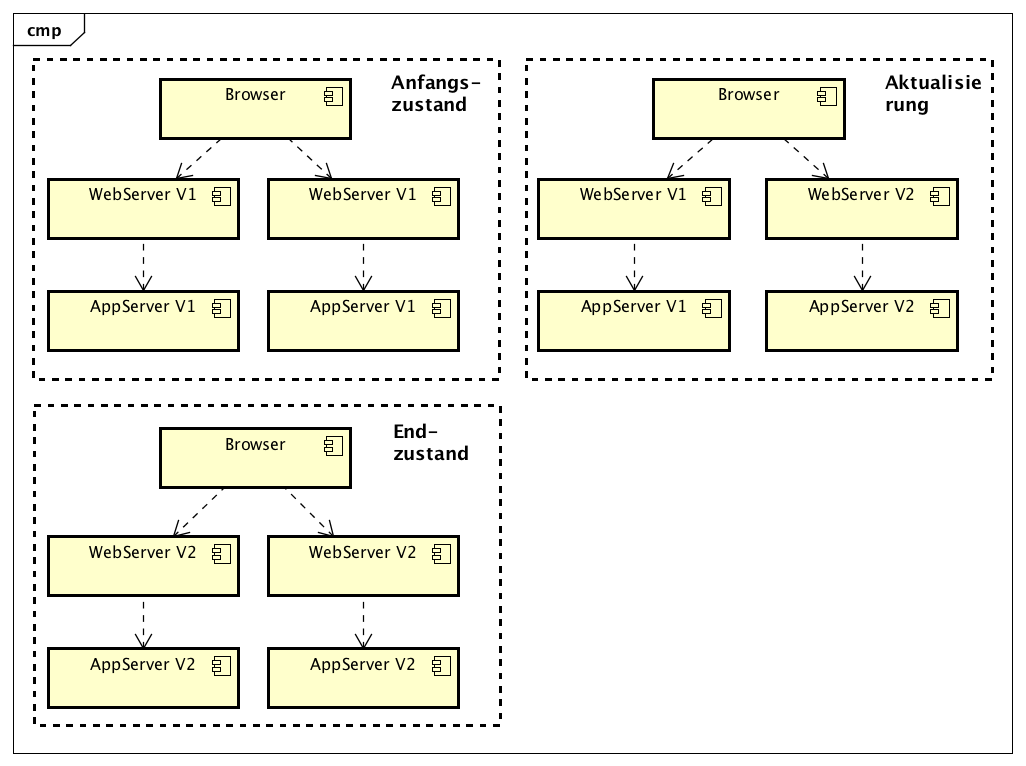
\includegraphics[scale=0.55]{MultiVersion.png}
\end{center}

Daraus lässt sich schliessen, dass die neue Architektur den gleichzeitigen Betrieb von mehreren Versionen unterstützen muss. Dies gilt vor allem für die Schnittstellen und die Datenspeicherung. Da die Applikation nicht geschäftskritisch ist, könnte die Aktualisierung auch in der Nacht durchgeführt werden wenn sich tendenziell kein Benutzer auf der Webseite befinden. So könnten die Probleme mit der Versionierung der Schnittstelle umgangen werden, für die Datenbank braucht es dennoch eine Lösung.	

\section{Teilprobleme}

Mit dem generellen Verständnis und den Anforderungen konnten nun die Teilprobleme identifiziert und entsprechende Lösungsvarianten gesucht werden. Diese sind in der Arc42 Vorlage nicht explizit ausgewiesen haben sich im Workshop des CAS Software Architektur als hilfreiches Mittel erwiesen das Gesamtproblem in kleinere aufzuteilen und wenn möglich austauschbare Lösungsvarianten zu erarbeiten.

\subsection{Versionierung}

Wie bereits in der Problematik erwähnt, müssen Schnittstellen versioniert werden und abwärts kompatibel sein damit der Benutzer von einer Änderung nichts merkt. Hier geht es vor allem um die REST Endpunkte welche der Onboarding Server der Webseite zur Verfügung stellt.

\subsection{Datenspeicherung}

Ebenfalls in der Problematik erwähnt, ist die Datenspeicherung. Aktuell wird für die Applikation eine relationale Datenbank verwendet. Die Datenbanken habe ein definiertes Schema welche Datentypen in den entsprechenden Feldern abgelegt werden dürfen und wie die Tabellen miteinander in Beziehung stehen. Hier stellt sich die Frage ob es Lösungen gibt welche den weiteren Einsatz der Technologie erlauben unter der Berücksichtigung der zusätzlichen Anforderung der Replikation. Soll die Applikation unterbruchsfrei aktualisiert werden können, muss die Datenbank hochverfügbar sein und automatische Mechanismen für den Fehlerfall bereitstellen.

\subsection{Kommunikationsentkopplung}

Soll der Benutzer sich auch bei der Aktualisierung der Applikation für TWINT registieren können, dürfen die Anfragen nicht verloren gehen respektive ein Fehler auftreten wenn eine Komponente wegen dem Update nicht verfügbar ist. Dies gilt vor allem zwischen Onboarding Server und der Workflow Engine. Obschon diese wie bereits erwähnt selber nicht berücksichtigt wird, sind die Schnittstellen zur Engine davon betroffen.

\subsection{Konfigurationsmanagement}

Im Ist-Zustand wurde das aktuelle Konfigurationsmanagement mittels Docker und Docker Compose bereits erwähnt. Für die neuen Anforderungen muss die aktuelle Lösung geprüft und gegebenenfalls ein andere Ansatz verfolgt werden. Die Änderung der Konfiguration zur Laufzeit als neue Anforderung ist bei einer Applikation die immer wieder ausgerollt werden soll, zwingend notwending um die einzelnen Funktionen besser steuern zu können.

\subsection{Deployment Pipeline}

Die Build Pipeline\footnote{Eine Pipeline ist eine Abfolge von Buildäufträgen(Stages) welche parallel und sequenziell ablaufen können. } welche im Antrag erwähnt wurde wegen ihrer Wichtigkeit für das Bauen und Installieren der Applikation wurde nicht weiterverfolgt. Der Grund darin liegt in dem Fortschritt der Methodik welche das Projekt seit dem Antrag gemacht hat. Wie in\cite{atlassiancd} beschrieben, sind verschieden Stages in der Pipeline sowie Feature Brachens in GIT eine Voraussetzung um eine Applikation zeitnahe in Betrieb zu bringen. Diese Praktiken werden aktuell im normalen Arbeitstag verwendet und müssen deshalb nicht nochmals evaluiert werden.

\section{Bewertungskriterien}

Die auszuarbeitenden Lösungsvarianten müssen auf ihre Verwendbarkeit geprüft und bewertet werden. Obschon Qualitätsziele für die Architektur definiert sind, eignen sie sich für die Bewertung von Bibliotheken und Lösungsvarianten nur bedingt. Weder das Arc42 Template noch \cite{esa} haben angemessen Metriken und Methoden im Angebot. Aus diesem Grund wird eine Bewertungsmatrix erstelle welche im CAS Software Architkur Workshop Modul bereits angewendet wurde. Dabei sind die einzelnen Kriterien mit dem Product Owner abgesprochen und gewichtet worden. Dabei lag der Fokus mehr auf Eigenschaften der Einzelnen Bibliotheken und Produkte wie Maturität, vorhandenes Wissen, oder auf Aufwand. Die Kriterien überlappen sich an einigen Stellen mit den Qualitätszielen was jedoch nicht als Nachteil gewertet wurde. Die Kritieren sind gezielt vor der Lösungsfindung erstellt worden, sodass diese zu stark durch die Variante beeinflusst wurden. Spätere Anpassungen mussten trotzdem gemacht werden da nicht alles von Beginn an klar war. Die Kriterien für sind im SAD im Kapitel 9.2 detailiert aufgeführt.

\section{Teillösungen}

Diverse Teilösungen indentifiziert anhand der bis zu diesem Zeitpunkt vorhandenen Requirements -> Qualitätsziele nach wievor nicht komplett klar.
Möglichst grosser Lösungsraum an Teilprobleme um eine gute Sicht auf das zu lösende Problem zu bekommen.

Prototypen erstellen für die Unklarheiten der ausgewählen Teillösungen.

Bild erstellen für Problem der Datenmigration resp. der unterstützung von zwei gleichzeitig laufenden versionen.
RDBMS -> trigger recursion, migration
NoSQL -> kein schema jedoch gleiches problem

CAP Theorem

MySQL CA, Mongo CP

Beide Datenbankentypen erlauben das Problem zu lösen. RDBMS braucht die ändernung an zwei stellen-> Buch über alle möglichen Variationen. Zyrkuläre Trigger tükisch. Mongo: alle muss in Code gemacht werden. Ermöglich schrittweise migration


Evaluation Graphql
Content Negogiation und Versionierung nicht im Prototyp abgebildet da bereits hinreichend bekannt.
Graphql sehr mühesam für Mutationen nicht die gleiche Konfiguration wie für die Abfragen verwendet werden kann.Übergabe wie MAp was sehr viel casten verursacht.. Library nicht von einer Organisation entwickelt sondern von 36 Entwicklern über Github. Gelegentliche Commits jedoch nicht wirk lebendig. 

Erweitern der Bewerungskriterien anhan der erkenntnisse aus den Prototypen.

\section{Lösungsvariante}

MongoDB, OpenShift Spring Cloud Config, Spring Bus

\section{Prototyp}

\section{Bewertung}

https://www.innoq.com/de/blog/why-restful-communication-between-microservices-can-be-perfectly-fine/

http://microservices.io/patterns/microservices.html

http://scs-architecture.org/vs-ms.html

http://de.slideshare.net/ewolff/rest-vs-messaging-for-microservices

https://www.symfony.fi/entry/versioning-an-api-in-graphql-vs-rest

https://redis.io/commands/rpoplpush

https://redis.io/topics/replication

http://blog.kubernetes.io/2016/04/configuration-management-with-containers.html

https://docs.mongodb.com/v3.2/replication/

https://dzone.com/articles/netflix-oss-spring-cloud-or-kubernetes-how-about-a

http://stackoverflow.com/questions/35998227/can-i-use-kubernetes-as-service-discovery-in-spring-cloud

https://developers.redhat.com/blog/2016/12/09/spring-cloud-for-microservices-compared-to-kubernetes/

http://de.slideshare.net/ewolff/rest-vs-messaging-for-microservices

https://www.innoq.com/de/blog/why-restful-communication-between-microservices-can-be-perfectly-fine/

https://vimeo.com/144746079

https://spring.io/guides/gs/messaging-redis/

https://seanmcgary.com/posts/how-to-build-a-fault-tolerant-redis-cluster-with-sentinel

https://spring.io/guides/gs/centralized-configuration/

https://wiki.jenkins-ci.org/display/JENKINS/zap+plugin

https://www.digitalocean.com/community/tutorials/how-to-create-a-multi-node-mysql-cluster-on-ubuntu-16-04

https://dev.mysql.com/doc/mysql-utilities/1.5/en/utils-task-autofailover.html

\url{https://docs.openshift.com/online/cli_reference/get_started_cli.html}

https://spring.io/guides/gs/spring-boot-docker/

\url{https://docs.openshift.com/online/cli_reference/get_started_cli.html}

https://github.com/OpenShiftDemos/openshift-cd-demo

http://www.sohamkamani.com/blog/2016/06/30/docker-mongo-replica-set/

\url{https://docs.openshift.com/online/using_images/db_images/mysql.html#using-mysql-replication}

https://blog.openshift.com/openshift-3-demo-part-8-rolling-deployments/

http://docs.spring.io/spring-boot/docs/current/reference/html/howto-database-initialization.html

http://dev.mysql.com/doc/refman/5.7/en/trigger-syntax.html

\url{http://mongodb.github.io/mongo-csharp-driver/2.3/reference/bson/mapping/schema_changes/}

\url{https://www.mongodb.com/blog/post/6-rules-of-thumb-for-mongodb-schema-design-part-1}

\url{https://www.mongodb.com/blog/post/6-rules-of-thumb-for-mongodb-schema-design-part-2}

\url{https://www.mongodb.com/blog/post/6-rules-of-thumb-for-mongodb-schema-design-part-3}

https://github.com/graphql-java/todomvc-relay-java

https://github.com/graphql-java/graphql-java

http://www.sohamkamani.com/blog/2016/06/30/docker-mongo-replica-set/

https://kubernetes.io/docs/user-guide/pods/









